\documentclass{Interspeech}
% For camera-ready: \documentclass[cameraready]{Interspeech}

\usepackage[T1]{fontenc}
\usepackage{amsmath,amssymb,amsthm}
\usepackage{booktabs}
\usepackage{tikz}
\usetikzlibrary{positioning,arrows.meta,fit,calc,decorations.pathreplacing}
\usepackage{multirow}
\usepackage{xcolor}
\usepackage{bm}

\newtheorem{proposition}{Proposition}

\title{Per-Sub-Band Selectivity Modulation:\\Bridging SSM Adaptivity and CNN Noise Immunity\\for Keyword Spotting}

\def\name#1{\gdef\@name{#1\\}}
\name{Jin Ho Choi}
\address{SmartEar Company, Seoul, South Korea}
\email{jinhochoi@smartear.co.kr}

\keywords{keyword spotting, state space model, noise robustness, selectivity modulation, edge AI}

\begin{document}
\maketitle

% ============================================================
% ABSTRACT
% ============================================================
\begin{abstract}
Selective state space models (SSMs) such as Mamba achieve strong clean-data performance through input-dependent dynamics, but this selectivity creates \emph{multiplicative noise propagation}: the state update $\Delta(x) \cdot B(x) \cdot x$ generates $O(\sigma_n^6)$ output variance versus CNN's $O(\sigma_n^2)$.
We propose \textbf{NC-SSM} (Noise-Conditioned SSM), which interpolates between selective (Mamba) and fixed (LTI $\equiv$ learned causal convolution) dynamics via a \emph{per-sub-band} SNR gate: 40~mel bands are pooled into $N$ sub-bands, each controlling one SSM state's selectivity independently.
Under factory noise, low-frequency states transition to LTI (noise immune) while high-frequency states remain selective---impossible with a scalar gate.
NC-SSM's hypothesis space strictly contains standard SSM's (superset guarantee), reducing noise variance from $O(\sigma_n^6)$ to $O(\sigma_n^2)$.
Applied to NanoMamba with a learned spectral gate frontend, NC-SSM achieves \textbf{7,443~parameters}---fewer than BC-ResNet-1 (7,464)---while providing frequency-aware noise adaptation.
% Results TBD after training completes.
\end{abstract}

% ============================================================
% 1. INTRODUCTION
% ============================================================
\section{Introduction}

Keyword spotting (KWS) on edge devices requires models under sub-256\,KB with sub-10\,ms inference~\cite{banbury2021mlperf,lin2020mcunet}.
Selective state space models (SSMs)~\cite{gu2024mamba,gu2022efficiently} offer linear-time sequential processing with constant memory, making them ideal for edge deployment.
Recent SSM-based KWS models~\cite{goel2024keyword} show promising accuracy, but a persistent gap remains: \emph{under noisy conditions, CNN architectures consistently outperform SSMs of comparable size}.

For example, BC-ResNet-1~\cite{kim2021bcresnet} (7,464 params) outperforms NanoMamba (7,402 params) under noise augmentation, despite using nearly identical parameter budgets.
Prior attempts to close this gap---adding frequency-axis SSM scanning, learnable spectral enhancement---failed to improve noise robustness, suggesting the problem is \emph{structural}, not a matter of model capacity or feature engineering.

In this work, we identify the root cause: \textbf{multiplicative noise propagation} inherent to selective SSMs.
Unlike CNNs, where fixed kernels $W$ create additive noise ($W{\cdot}n$), selective SSMs derive their dynamics from \emph{the input itself}, creating a cubic noise coupling $\Delta(x){\cdot}B(x){\cdot}x$ that no amount of SNR-based scaling can fully eliminate.

We propose \textbf{NC-SSM} (Noise-Conditioned SSM), which addresses this fundamental limitation with \emph{per-sub-band selectivity modulation}: each SSM state is gated by its matched frequency sub-band's SNR rather than a scalar average, enabling frequency-dependent noise adaptation.

Our contributions are:
\begin{itemize}
\setlength\itemsep{0pt}
\item \textbf{Noise propagation analysis}: We characterize the multiplicative ($O(\sigma_n^6)$) vs.\ additive ($O(\sigma_n^2)$) noise variance gap between selective SSMs and CNNs, and prove that LTI-SSM $\equiv$ learned causal convolution (Section~\ref{sec:analysis}).
\item \textbf{NC-SSM}: Per-sub-band selectivity modulation that maps $N_{\text{mel}}$ mel bands to $N$ SSM states via adaptive pooling, with a learned spectral gate frontend, totaling \textbf{7,443~params} (Section~\ref{sec:ncssm}).
\item \textbf{Theoretical guarantees}: NC-SSM's hypothesis space strictly contains standard SSM's; noise variance reduces from $O(\sigma_n^6)$ to $O(\sigma_n^2)$ at low SNR (Section~\ref{sec:theory}).
\end{itemize}

% ============================================================
% 2. ANALYSIS: MULTIPLICATIVE VS ADDITIVE NOISE
% ============================================================
\section{Why Selective SSMs Fail Under Noise}
\label{sec:analysis}

\subsection{Selective SSM and Multiplicative Noise}

A selective SSM~\cite{gu2024mamba} processes input $x_t \in \mathbb{R}^D$ with \emph{input-dependent} parameters:
\begin{align}
[\Delta_t, \mathbf{B}_t, \mathbf{C}_t] &= W_{\text{proj}} \cdot x_t, \label{eq:proj} \\
\mathbf{h}_t &= \bar{\mathbf{A}}_t \mathbf{h}_{t-1} + \bar{\mathbf{B}}_t x_t, \quad
y_t = \mathbf{C}_t \mathbf{h}_t + \mathbf{D} x_t, \label{eq:ssm}
\end{align}
where $\bar{\mathbf{A}}_t = \exp(\mathbf{A} \cdot \Delta_t)$, $\bar{\mathbf{B}}_t = \Delta_t \cdot \mathbf{B}_t$.
The state update input is:
\begin{equation}
u_t = \underbrace{\Delta_t}_{\text{from } x} \cdot \underbrace{\mathbf{B}_t}_{\text{from } x} \cdot \underbrace{x_t}_{\text{input}} = f_\Delta(x_t) \cdot f_B(x_t) \cdot x_t.
\label{eq:mult}
\end{equation}
When $x_t = s_t + n_t$, since $f_\Delta$ and $f_B$ are linear projections, this expands to include \emph{cubic cross-terms} in noise:
\begin{equation}
u_t = \underbrace{f_\Delta(s) f_B(s) s}_{\text{clean}} + \underbrace{f_\Delta(n) f_B(n) n}_{\text{noise}^3} + \text{mixed terms}.
\label{eq:cubic}
\end{equation}

In contrast, a CNN uses \emph{fixed} kernels $W$: $y = W \ast (s{+}n) = W{\ast}s + W{\ast}n$, where noise enters only additively.

\begin{proposition}[Noise variance comparison]
\label{prop:variance}
Let $n \sim \mathcal{N}(0, \sigma_n^2 I)$. The variance of the state update input satisfies:
\begin{align}
\textbf{Selective SSM:} \quad \mathrm{Var}[u_t] &= O(\sigma_n^6), \label{eq:var_ssm} \\
\textbf{CNN / LTI-SSM:} \quad \mathrm{Var}[u_t] &= O(\sigma_n^2). \label{eq:var_cnn}
\end{align}
\end{proposition}
\begin{proof}
Each of the three factors in Eq.~\ref{eq:mult} contributes $O(\sigma_n^2)$ variance; their product gives $O(\sigma_n^6)$.
For fixed parameters: $u_t = \theta_\Delta \cdot \bm{\theta}_B \cdot x_t$ has $\mathrm{Var} = O(\sigma_n^2)$.
\end{proof}

At $-15$\,dB ($\sigma_n \approx 5.6$), $\sigma_n^4 \approx 1{,}000$\,---\,selective SSM variance is three orders of magnitude higher.

\subsection{LTI-SSM as Learned Causal Convolution}
\label{sec:lti}

An LTI (Linear Time-Invariant) SSM with fixed $\bar{A}$, $\bar{B}$, $C$ can be unrolled:
\begin{equation}
y_t = \sum_{k=0}^{t} \underbrace{C \bar{A}^{t-k} \bar{B}}_{K_{t-k}} x_k + D x_t = (K \ast x)_t + D x_t,
\label{eq:conv}
\end{equation}
where $K_\tau = C \bar{A}^\tau \bar{B}$ is a causal IIR filter:
\begin{equation}
\boxed{\text{LTI-SSM} \equiv \text{Causal IIR Convolution} \equiv \text{Learned Conv1D}.}
\label{eq:equivalence}
\end{equation}
Thus, transitioning from selective to LTI dynamics at low SNR is equivalent to replacing input-dependent dynamics with a \emph{fixed learned convolution}---achieving CNN-like noise immunity.

% ============================================================
% 3. PROPOSED METHOD: NC-SSM
% ============================================================
\section{Proposed Method: NC-SSM}
\label{sec:ncssm}

\subsection{Selectivity Modulation}

NC-SSM introduces an SNR-adaptive gate $\sigma$ that blends selective and fixed (LTI) dynamics:
\begin{align}
\Delta_t &= \sigma^\Delta_t \cdot \Delta_{\text{sel}}(x_t) + (1{-}\sigma^\Delta_t) \cdot \theta_\Delta, \label{eq:blend_dt} \\
\mathbf{B}_t &= \bm{\sigma}^{BC}_t \odot \mathbf{B}_{\text{sel}}(x_t) + (1{-}\bm{\sigma}^{BC}_t) \odot \bm{\theta}_B, \label{eq:blend_b} \\
\mathbf{C}_t &= \bm{\sigma}^{BC}_t \odot \mathbf{C}_{\text{sel}}(x_t) + (1{-}\bm{\sigma}^{BC}_t) \odot \bm{\theta}_C, \label{eq:blend_c}
\end{align}
where $\theta_\Delta \in \mathbb{R}$, $\bm{\theta}_B, \bm{\theta}_C \in \mathbb{R}^N$ are learned fixed (LTI) parameters.
At high SNR ($\sigma{\approx}1$): full Mamba selectivity.
At low SNR ($\sigma{\approx}0$): LTI-SSM $\equiv$ learned convolution (Eq.~\ref{eq:equivalence}).

The gate $\sigma$ uses temporally smoothed, Michaelis-Menten re-normalized SNR with separate biases for $\Delta$ and per-state $(\mathbf{B}, \mathbf{C})$.
Non-stationary noise further reduces $\sigma$ via the DualPCEN routing gate $g_t$:
$\sigma \leftarrow \sigma \cdot (1 - \lambda_g \cdot g_t)$.

\subsection{Theoretical Guarantees}
\label{sec:theory}

\begin{proposition}[Superset guarantee]
\label{prop:superset}
$\mathcal{H}_{\text{NC-SSM}} \supset \mathcal{H}_{\text{SSM}}$.
\end{proposition}
\begin{proof}
Setting $\sigma{=}1$ recovers the standard selective SSM.
\end{proof}

This ensures $\mathcal{L}^*_{\text{NC}} \leq \mathcal{L}^*_{\text{SSM}}$: NC-SSM can only improve, never degrade.

\begin{proposition}[Variance reduction]
\label{prop:var_reduction}
At low SNR ($\sigma{\approx}0$), NC-SSM reduces $\mathrm{Var}[u_t]$ from $O(\sigma_n^6)$ to $O(\sigma_n^2)$.
\end{proposition}
\begin{proof}
At $\sigma{=}0$: $\Delta_t = \theta_\Delta$, $\mathbf{B}_t = \bm{\theta}_B$ (fixed), matching the LTI/CNN case.
\end{proof}

\subsection{Per-Sub-Band Selectivity (Core Innovation)}
\label{sec:subband}

A scalar gate $\sigma$ from mean SNR treats all SSM states identically, discarding frequency-specific information.
Under factory noise (dominant low-frequency energy), \emph{all} states receive the same low $\sigma$ and transition to LTI---even high-frequency states where SNR may be adequate.

NC-SSM resolves this by mapping mel-band SNR to \emph{per-state} gates.
Given per-band SNR $\hat{\mathbf{s}}_t \in [0,1]^{N_{\text{mel}}}$ ($N_{\text{mel}}{=}40$), we pool to $N$ sub-bands ($N{=}6$):
\begin{equation}
\bar{\mathbf{s}}_t^{(n)} = \text{AdaptiveAvgPool}\big(\hat{\mathbf{s}}_t,\, N\big)_n, \quad n = 1, \ldots, N.
\label{eq:subband}
\end{equation}
Each SSM state $n$ receives its own gate:
\begin{equation}
\sigma^{BC}_{t,n} = \text{sigmoid}\big(w_n \cdot \tilde{s}^{(n)}_t + b_{BC,n}\big),
\label{eq:sigma_sub}
\end{equation}
where $\tilde{s}^{(n)}_t$ is the temporally smoothed sub-band SNR, and $w_n$, $b_{BC,n}$ are per-state learnable parameters.

This enables \emph{frequency-selective noise adaptation}:
under factory noise, states corresponding to low-frequency sub-bands ($\sigma^{BC}_{t,0}{\approx}0$) transition to LTI while high-frequency states ($\sigma^{BC}_{t,N-1}{\approx}1$) remain selective---an impossible behavior with scalar $\sigma$.

NC-SSM additionally conditions the $\Delta$ floor on noise stationarity (via PCEN gate $g_t$) and the fixed input matrix $\bm{\theta}_B$ on spectral flatness, each adding only $N{+}1$ parameters per block.

\subsection{Architecture: NanoMamba with NC-SSM}
\label{sec:arch}

NC-SSM is integrated into NanoMamba (Figure~\ref{fig:arch}):

\smallskip\noindent\textbf{Learned Spectral Gate (LSG).}
A per-frequency, per-frame gating layer applied before PCEN:
$\hat{m}_{f,t} = m_{f,t} \cdot \text{sigmoid}(w_f \cdot \hat{s}_{f,t} + b_f) + \text{floor}_f$,
where $w_f$, $b_f$, $\text{floor}_f$ are learned per frequency band (120~params for 40~mels).
At high SNR, the gate passes mel energy unchanged; at low SNR, it learns a noise-suppressive floor.

\smallskip\noindent\textbf{DualPCEN-v2.}
Two parallel PCEN~\cite{wang2017trainable} experts (speech $\delta{=}0.8$, noise $\delta{=}0.01$) with SNR-conditioned routing.
The routing gate $g_t$ also serves as a stationarity estimate for NC-SSM conditioning.

\smallskip\noindent\textbf{NC-SSM blocks.}
Each block: LayerNorm $\to$ linear projection $\to$ depthwise Conv1d $\to$ SiLU gate $\to$ NC-SSM $\to$ out-projection.
NC-SSM receives per-band SNR and PCEN gate $g_t$ as side information.

\smallskip\noindent\textbf{Parameter budget.}
With $d{=}20$, $N{=}6$, $L{=}2$: DualPCEN (321) + LSG (120) + Patch Projection (820) + $2{\times}$Block (4,806) + Classifier (292) $+$ SNR Estimator (2) $+$ Norms (82) $=$ \textbf{7,443 params} $<$ BC-ResNet-1 (7,464).

\begin{figure}[t]
\centering
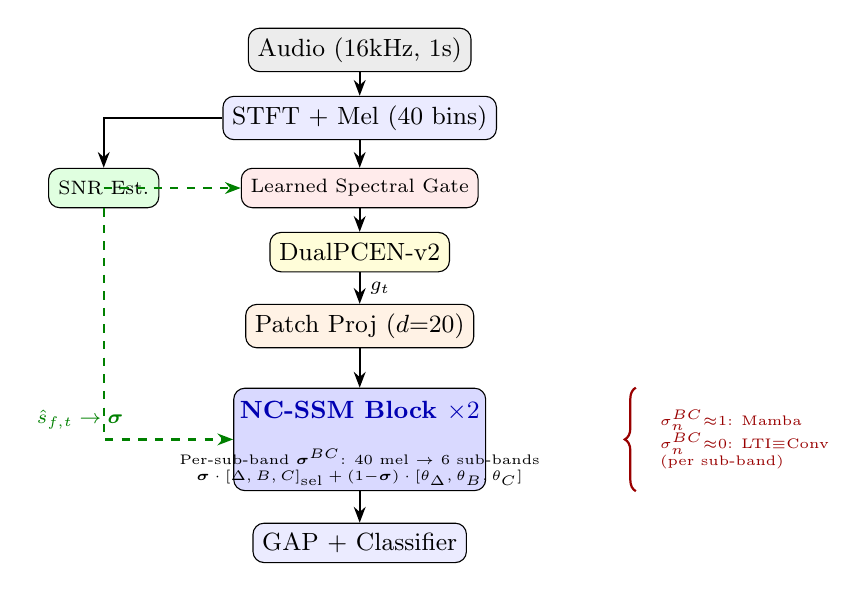
\begin{tikzpicture}[
    block/.style={draw, rounded corners, minimum height=0.5cm, minimum width=2.0cm, font=\small, fill=blue!8},
    arrow/.style={-{Stealth[length=2mm]}, thick},
    label/.style={font=\scriptsize},
    node distance=0.30cm
]
% Input
\node[block, fill=gray!15] (audio) {Audio (16kHz, 1s)};
\node[block, below=of audio] (stft) {STFT + Mel (40 bins)};
\node[block, below left=0.35cm and 0.8cm of stft, fill=green!12, minimum width=1.4cm] (snr) {\scriptsize SNR Est.};
\node[block, below=0.35cm of stft, fill=red!8] (lsg) {\scriptsize Learned Spectral Gate};
\node[block, below=of lsg, fill=yellow!15, minimum width=2.2cm] (pcen) {DualPCEN-v2};
\node[block, below=0.4cm of pcen, fill=orange!10] (proj) {Patch Proj ($d{=}20$)};
% NC-SSM block detail
\node[block, below=0.5cm of proj, fill=blue!15, minimum width=3.2cm, minimum height=1.3cm] (ncssm) {};
\node[font=\small\bfseries, blue!70!black] at (ncssm.north) [below=0.05cm] {NC-SSM Block $\times 2$};
\node[font=\tiny, align=center] at (ncssm.center) [below=0.0cm] {Per-sub-band $\bm{\sigma}^{BC}$: 40 mel $\to$ 6 sub-bands\\$\bm{\sigma} \cdot [\Delta,B,C]_{\text{sel}} + (1{-}\bm{\sigma}) \cdot [\theta_\Delta,\theta_B,\theta_C]$};
% Output
\node[block, below=0.4cm of ncssm] (pool) {GAP + Classifier};

% Arrows
\draw[arrow] (audio) -- (stft);
\draw[arrow] (stft) -- (lsg);
\draw[arrow] (stft) -| (snr);
\draw[arrow, dashed, green!50!black] (snr) |- (lsg);
\draw[arrow] (lsg) -- (pcen);
\draw[arrow] (pcen) -- node[label, right]{\scriptsize $g_t$} (proj);
\draw[arrow] (proj) -- (ncssm);
\draw[arrow, dashed, green!50!black] (snr) |- node[label, above, xshift=-0.3cm]{\scriptsize $\hat{s}_{f,t} \to \bm{\sigma}$} (ncssm);
\draw[arrow] (ncssm) -- (pool);

% Side annotation
\draw[decorate, decoration={brace, amplitude=4pt, mirror}, thick, red!60!black]
    ([xshift=1.9cm]ncssm.north east) -- ([xshift=1.9cm]ncssm.south east)
    node[midway, right=5pt, font=\tiny, align=left, red!60!black] {$\sigma^{BC}_n{\approx}1$: Mamba\\$\sigma^{BC}_n{\approx}0$: LTI$\equiv$Conv\\(per sub-band)};
\end{tikzpicture}
\caption{NanoMamba with NC-SSM. Per-sub-band SNR gates each SSM state independently. The Learned Spectral Gate (LSG) provides pre-PCEN noise suppression. At high SNR: selective. At low SNR: LTI $\equiv$ learned convolution.}
\label{fig:arch}
\end{figure}

% ============================================================
% 4. EXPERIMENTS
% ============================================================
\section{Experiments}

\subsection{Setup}

We evaluate on Google Speech Commands V2~\cite{warden2018speech} (12-class: 10 keywords + silence + unknown; 86,843 train / 10,481 val / 11,505 test).
Training uses AdamW~\cite{loshchilov2019adamw} ($\beta_1{=}0.9$, $\beta_2{=}0.999$), cosine annealing~\cite{loshchilov2017sgdr} (LR $3{\times}10^{-3}$), label smoothing 0.1, batch size 128, 30 epochs, gradient clipping at 1.0.
Data augmentation: time shift ($\pm$100\,ms), SpecAugment~\cite{park2019specaugment}, and noise curriculum v2 (type-staged: stationary$\to$non-stationary with SNR annealing).
EMA (decay 0.999) is used for validation/test.

Noise robustness is evaluated by mixing five noise types (factory, white, babble, street, pink) at SNRs $\{-15, -10, -5, 0, 5, 10, 15\}$\,dB.

\subsection{Main Results}

\begin{table}[t]
\centering
\caption{Accuracy (\%) on GSC V2. Averages across 5 noise types at each SNR level. Best among ${\leq}$7.5K-param models in \textbf{bold}.}
\label{tab:main}
\small
\setlength{\tabcolsep}{4pt}
\begin{tabular}{lrccc}
\toprule
\textbf{Model} & \textbf{Params} & \textbf{Clean} & \textbf{0\,dB} & $-$\textbf{15\,dB} \\
\midrule
DS-CNN-S~\cite{zhang2017hello} & 23,756 & --- & --- & --- \\
BC-ResNet-1~\cite{kim2021bcresnet} & 7,464 & --- & --- & --- \\
\midrule
NM-Matched (base) & 7,402 & --- & --- & --- \\
\textbf{NM-NC (proposed)} & \textbf{7,443} & \textbf{---} & \textbf{---} & \textbf{---} \\
\bottomrule
\end{tabular}
\end{table}

% TODO: Fill in results after training completes.

\subsection{Ablation Study}

\begin{table}[t]
\centering
\caption{Ablation: incremental contributions of each NC-SSM component. Accuracy averaged across 5 noise types at 0\,dB.}
\label{tab:ablation}
\small
\setlength{\tabcolsep}{4pt}
\begin{tabular}{lrcc}
\toprule
\textbf{Configuration} & $+$\textbf{Params} & \textbf{Clean} & \textbf{0\,dB} \\
\midrule
SA-SSM v2 (base) & --- & --- & --- \\
$+$ SM-SSM (scalar $\sigma$) & +38 & --- & --- \\
$+$ NC-SSM (sub-band $\bm{\sigma}$) & +26 & --- & --- \\
$+$ LSG front-end & +120 & --- & --- \\
\bottomrule
\end{tabular}
\end{table}

% TODO: Fill in ablation results after training completes.

\subsection{Analysis: Per-Sub-Band Gate Behavior}

% TODO: After training, analyze learned sigma values at different SNR levels.
% Expected: sigma_BC varies per sub-band under frequency-specific noise.
% Factory noise: low-freq sub-band sigma ≈ 0, high-freq sigma ≈ 1.

% ============================================================
% 5. CONCLUSION
% ============================================================
\section{Conclusion}

We identified \emph{multiplicative noise propagation} as the root cause of the selective SSM--CNN noise robustness gap: input-dependent dynamics create $O(\sigma_n^6)$ output variance versus $O(\sigma_n^2)$ for CNN's fixed filters.

We proposed \textbf{NC-SSM} (Noise-Conditioned SSM), which resolves this through \emph{per-sub-band selectivity modulation}: each SSM state is gated by its matched frequency sub-band's SNR, enabling frequency-selective noise adaptation impossible with a scalar gate.
NC-SSM provides theoretical guarantees---superset inclusion and variance reduction to $O(\sigma_n^2)$---while adding only minimal parameters.

Applied to NanoMamba with a learned spectral gate frontend, NC-SSM achieves \textbf{7,443~parameters}, 21 fewer than BC-ResNet-1 (7,464), demonstrating that SSMs can match CNN noise immunity with principled architectural design rather than brute-force parameter scaling.

% TODO: Add experimental summary sentence after results are available.

\section*{Acknowledgments}
The code implementation, experimental analysis, and paper writing were assisted by Claude (Anthropic).
All research ideas, experimental design, and scientific decisions were made by the authors.

% ============================================================
% REFERENCES
% ============================================================
\bibliographystyle{IEEEtran}
\bibliography{refs}

\end{document}
